\section{Ensemble Methods}
The main idea of ensemble is to combine algorithms to achieve a better accuracy than with a single model. Ensemble methods can be split into heterogeneous and homogeneous ensembles. In homogeneous ensembles only one classifier is used, while in heterogeneous ensembles different algorithms can be combined. 
We implemented a homogeneous method called AdaBoost with decision tree stumps (depth=1). This is a boosting method. There are other fields like Bagging (Bootstraping) or Random Forest which are not explained here. For a first introduction with Desicion Trees you can look at https://medium.com/analytics-vidhya/ensemble-methods-for-decision-trees-f4a658af754d.\\
\begin{figure}[hbtp]
	\centering
	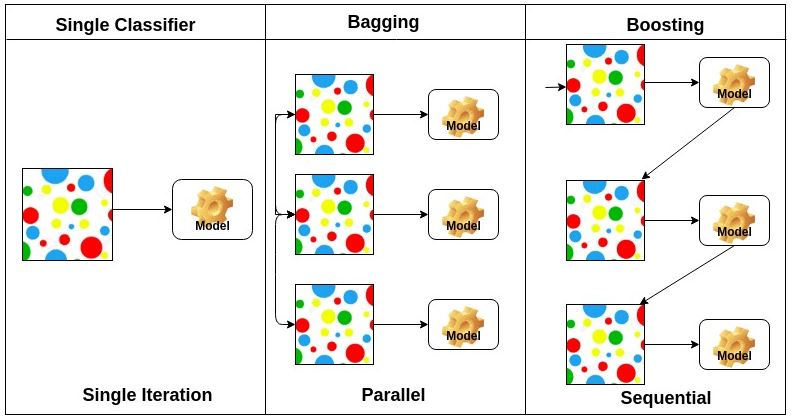
\includegraphics[scale=0.5]{ensemble_1}
	\caption{Bagging/Boosting}
	% \vspace{-20pt}
	\label{fig:Datensatz - unbearbeitet}
\end{figure}
If we consider decision trees, we can observe that they tend to overfit if they grow to their maximum depth. Also in every node there is uncertainty. Ensemble methods try to build a bunch of weak learner (like the mentioned stumps) to let them predict together and try to decrease variance (and bias).

%%%%%%%%%%%%%%%%%%%%%%%%%%%%%%%%%%%%%%%%%%%%%%%%%%%%%%%%%


\subsection{AdaBoost}
For our problem we implemented an algorithm called AdaBoost. The main idea behind AdaBoost is building a series of trees, each of those being an updated version of the previous one. At the end of the process, when all the classifiers built during the iterations will be asked to vote for the target of a new observation, there will be trees with a heavier vote than others. Those are the trees that performed the best during all the iterations (so, they showed very few misclassifications).

- AdaBoost works by putting more weight on difficult to classify instances and less on those already handled well.

Like mentioned we implemented AdaBoost with Stumps (depth=1). Regarding the functionality of Decision Trees we refer to Chapter 3 Classical learning. The input was the same like for the other algorithms (2304 pixels) and the emotions. The process of the algorithm can be seen in the following graphic. 
\begin{figure}[hbtp]
	\centering
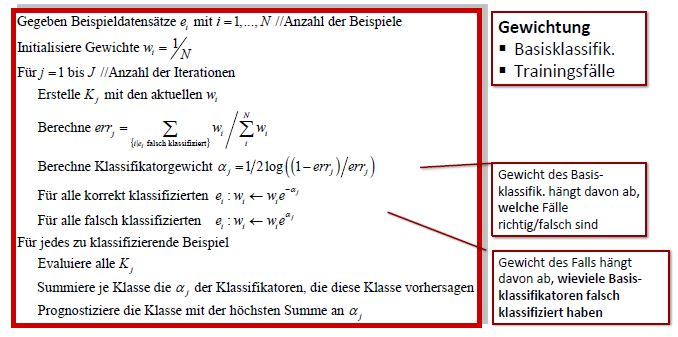
\includegraphics[scale=0.8]{Images/Adaboost_1.png} \\
\end{figure}

In summary it can be said that AdaBoost had a surprisingly good accuracy compared with SVM. But the algorithm tends to classify a lot of pictures as happy and is weak at classifying Angry, Disgust and Fear.\\
One advantage of AdaBoost is that it is easily implemented and the training is rather simple. It is also possible to use different weak learner (Trees, KNN, etc.) But if the weak learner selected doesn't fit the problem, then AdaBoost also struggles solving it. Also with growing iterations AdaBoost can overfit. Another disadvantage is that, due to the iterative calculation, it's difficult to parallelize.

\textbf{Sources:}
\begin{itemize}
\item Introduction to AdaBoost \hyperlink{https://towardsdatascience.com/understanding-adaboost-for-decision-tree-ff8f07d2851}{https://towardsdatascience.com/understanding-adaboost-for-decision-tree-ff8f07d2851}
\item scikit-learn: \hyperlink{https://scikit-learn.org/stable/modules/ensemble.html}{https://scikit-learn.org/stable/modules/ensemble.html} \\
\hyperlink{https://scikit-learn.org/stable/modules/generated/sklearn.ensemble.AdaBoostClassifier.html}{https://scikit-learn.org/stable/modules/generated/sklearn.ensemble.AdaBoostClassifier.html}
\item Video with an example \\ \hyperlink{https://www.youtube.com/watch?v=LsK-xG1cLYA}{https://www.youtube.com/watch?v=LsK-xG1cLYA}
\item Wikipedia: Boosting \hyperlink{https://de.wikipedia.org/wiki/Boosting}{https://de.wikipedia.org/wiki/Boosting}
\end{itemize}

%%%%%%%%%%%%%%%%%%%%%%%%%%%%%%%%%%%%%%%%%%%%%%%%%%%%%%%%%


\newpage